\documentclass{beamer}
\usepackage[utf8]{inputenc}

\usetheme{Boadilla}
\usecolortheme{lily}
\usepackage{amsmath,amssymb,amsfonts,amsthm}
\usepackage{mathtools}
\usepackage{txfonts}
\usepackage{tkz-euclide}
\usepackage{listings}
\usepackage{adjustbox}
\usepackage{array}
\usepackage{tabularx}
\usepackage{lmodern}
\usepackage{circuitikz}
\usepackage{tikz}
\usepackage{graphicx}

\setbeamertemplate{footline}
{
  \leavevmode%
  \hbox{%
  \begin{beamercolorbox}[wd=\paperwidth,ht=2.25ex,dp=1ex,right]{author in head/foot}%
    \insertframenumber{} / \inserttotalframenumber\hspace*{2ex} 
  \end{beamercolorbox}}%
  \vskip0pt%
}

\usepackage{tcolorbox}
\tcbuselibrary{minted,breakable,xparse,skins}




\providecommand{\nCr}[2]{\,^{#1}C_{#2}} % nCr
\providecommand{\nPr}[2]{\,^{#1}P_{#2}} % nPr
\providecommand{\mbf}{\mathbf}
\providecommand{\pr}[1]{\ensuremath{\Pr\left(#1\right)}}
\providecommand{\qfunc}[1]{\ensuremath{Q\left(#1\right)}}
\providecommand{\sbrak}[1]{\ensuremath{{}\left[#1\right]}}
\providecommand{\lsbrak}[1]{\ensuremath{{}\left[#1\right.}}
\providecommand{\rsbrak}[1]{\ensuremath{{}\left.#1\right]}}
\providecommand{\brak}[1]{\ensuremath{\left(#1\right)}}
\providecommand{\lbrak}[1]{\ensuremath{\left(#1\right.}}
\providecommand{\rbrak}[1]{\ensuremath{\left.#1\right)}}
\providecommand{\cbrak}[1]{\ensuremath{\left\{#1\right\}}}
\providecommand{\lcbrak}[1]{\ensuremath{\left\{#1\right.}}
\providecommand{\rcbrak}[1]{\ensuremath{\left.#1\right\}}}
\theoremstyle{remark}
\newtheorem{rem}{Remark}
\newcommand{\sgn}{\mathop{\mathrm{sgn}}}
\providecommand{\abs}[1]{\left\vert#1\right\vert}
\providecommand{\res}[1]{\Res\displaylimits_{#1}} 
\providecommand{\norm}[1]{\lVert#1\rVert}
\providecommand{\mtx}[1]{\mathbf{#1}}
\providecommand{\mean}[1]{E\left[ #1 \right]}
\providecommand{\fourier}{\overset{\mathcal{F}}{ \rightleftharpoons}}
%\providecommand{\hilbert}{\overset{\mathcal{H}}{ \rightleftharpoons}}
\providecommand{\system}{\overset{\mathcal{H}}{ \longleftrightarrow}}
	%\newcommand{\solution}[2]{\textbf{Solution:}{#1}}
%\newcommand{\solution}{\noindent \textbf{Solution: }}
\providecommand{\dec}[2]{\ensuremath{\overset{#1}{\underset{#2}{\gtrless}}}}
\newcommand{\myvec}[1]{\ensuremath{\begin{pmatrix}#1\end{pmatrix}}}
\let\vec\mathbf

\lstset{
%language=C,
frame=single, 
breaklines=true,
columns=fullflexible
}

\numberwithin{equation}{section}

\lstset{
  language=Python,
  basicstyle=\ttfamily\small,
  keywordstyle=\color{blue},
  stringstyle=\color{orange},
  numbers=left,
  numberstyle=\tiny\color{gray},
  breaklines=true,
  showstringspaces=false
}

\title{Problem 4.3.8}
\author{ee25btech11023-Venkata Sai}

\date{\today} 
\begin{document}

\begin{frame}
\titlepage
\end{frame}

\section*{Outline}
\begin{frame}
\tableofcontents
\end{frame}

\section{Problem}

\begin{frame}
\frametitle{Problem}
\setcounter{section}{1}
 The vector equation of the line
\begin{align}
\frac{x-5}{3} = \frac{y+4}{7} = \frac{z-6}{2}
\end{align}
is
\end{frame}
%\subsection{Literature}
\section{Solution}

\subsection{Finding $\vec{a}$ and $\vec{b}$}
\begin{frame}
\frametitle{Finding $\vec{a}$ and $\vec{b}$}
A point on the line  is given as
\begin{align}
\myvec{x-5 \\y+4 \\z-6}=\myvec{0\\0\\0}\\
\vec{a}=\myvec{x\\y\\z}=\myvec{5\\-4\\6}
\end{align}
The direction vectors of given line are
\begin{align}
    \vec{b}=\myvec{3\\7\\2}
\end{align}
\end{frame}
\subsection{Conclusion}
\begin{frame}
\frametitle{Conclusion}
 The vector equation of a line is given as
\begin{align}
    \vec{r}=\vec{a}+t\vec{b} 
    \end{align}
    \begin{align}
    \vec{r}=\myvec{5\\-4\\6}+t\myvec{3\\7\\2}
\end{align}
\end{frame}

\subsection{Plot}
\begin{frame}[fragile]
\frametitle{Plot}

\begin{figure}[h!]
   \centering
   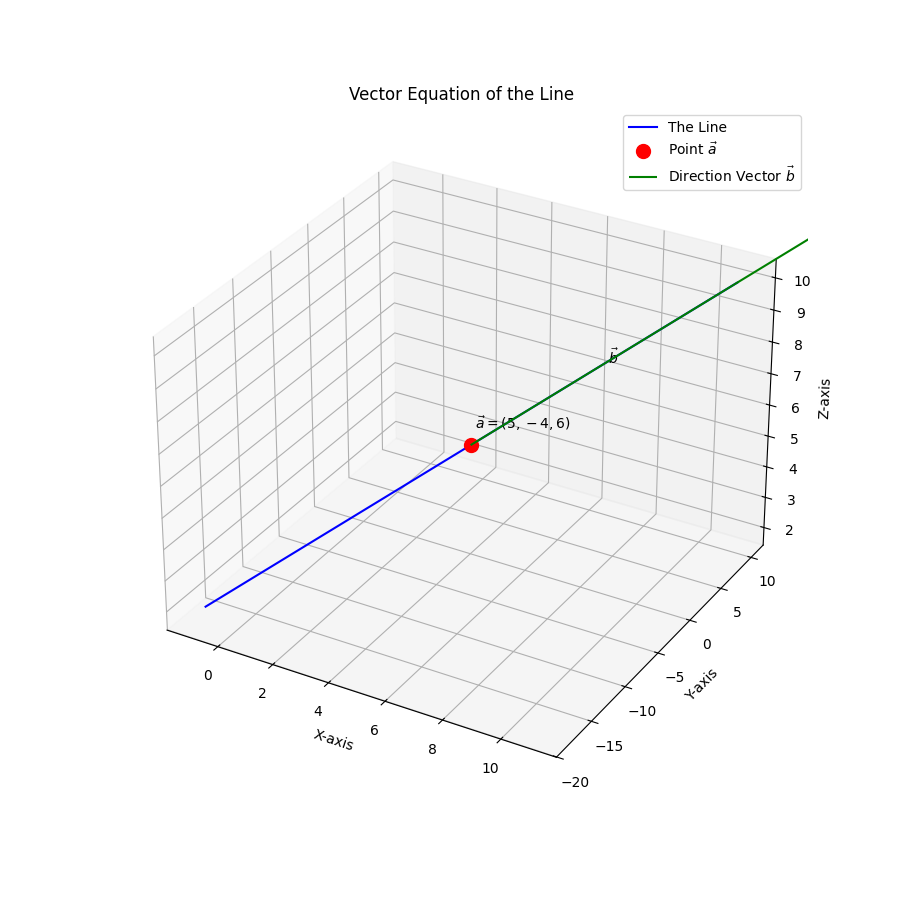
\includegraphics[width=0.7\columnwidth]{figs/fig1.png}
	\caption{}
   \label{}
\end{figure}
\end{frame}

\section{C Code}
\begin{frame}[fragile]
\frametitle{C Code}
\begin{lstlisting}[language=C]
void get_line_vectors(double* out_data) {
 
    double point_a[3] = {5.0, -4.0, 6.0};
    double dir_b[3] = {3.0, 7.0, 2.0};
    
    out_data[0] = point_a[0];
    out_data[1] = point_a[1];
    out_data[2] = point_a[2];
    
    out_data[3] = dir_b[0];
    out_data[4] = dir_b[1];
    out_data[5] = dir_b[2];
}
    \end{lstlisting}
\end{frame}
\section{Python Code}
\begin{frame}[fragile]
\frametitle{Calling C Function}
\begin{lstlisting}[language=Python]
import ctypes
import numpy as np

def get_vectors_from_c():
    lib = ctypes.CDLL('./vector.so')

    # The C function expects a pointer to a C double array of size 6
    double_array_6 = ctypes.c_double * 6
    lib.get_line_vectors.argtypes = [ctypes.POINTER(ctypes.c_double)]
    
    # Create the C-style array to receive the output data
    out_data_c = double_array_6()
    
    # Call the C function, which will fill the array
    lib.get_line_vectors(out_data_c)
\end{lstlisting}
\end{frame}
\begin{frame}[fragile]
\frametitle{Calling C Function}
\begin{lstlisting}[language=Python]
# Convert the C array back into a NumPy array
    all_data = np.array(out_data_c)
    
    # Split the data into the point vector and direction vector
    point_a = all_data[:3]
    dir_b = all_data[3:]
    
    return point_a, dir_b
    \end{lstlisting}
\end{frame}
\begin{frame}[fragile]
\frametitle{Python Code for Plotting}
\begin{lstlisting}[language=Python]
#Code by GVV Sharma
#September 12, 2023
#Revised July 21, 2024
#released under GNU GPL

import sys
import matplotlib.pyplot as plt
import numpy as np
from mpl_toolkits.mplot3d import Axes3D
sys.path.insert(0, '/workspaces/urban-potato/matgeo/codes/CoordGeo/') 
from call import get_vectors_from_c
hat_symbol = '\u0302'
from line.funcs import *
from triangle.funcs import *
from conics.funcs import circ_gen

point_a, dir_b = get_vectors_from_c()
 
\end{lstlisting}
\end{frame}

\begin{frame}[fragile]
\frametitle{Python Code for Plotting}
\begin{lstlisting}[language=Python]
from call import get_vectors_from_c

point_a, dir_b = get_vectors_from_c()
 
lambda_vals = np.array([-2, 2])
line_points = point_a + lambda_vals[:, np.newaxis] * dir_b

# --- Plotting ---
fig = plt.figure(figsize=(9, 9))
ax = fig.add_subplot(111, projection='3d')

# Plot the line segment itself
ax.plot(line_points[:, 0], line_points[:, 1], line_points[:, 2], color='blue', label='The Line')

# Plot the point 'a' on the line
ax.scatter(point_a[0], point_a[1], point_a[2], color='red', s=100, label='Point $\\vec{a}$')

\end{lstlisting}
\end{frame}

\begin{frame}[fragile]
\frametitle{Python Code for Plotting}
\begin{lstlisting}[language=Python]
  # Plot the direction vector 'd' starting from point 'a'
ax.quiver(point_a[0], point_a[1], point_a[2], 
          dir_b[0], dir_b[1], dir_b[2], 
          color='green', label='Direction Vector $\\vec{b}$', length=5, arrow_length_ratio=0.3)

# Add text labels for the point and vectors
ax.text(point_a[0], point_a[1], point_a[2] + 0.5, f' $\\vec{{a}} = ({point_a[0]:.0f}, {point_a[1]:.0f}, {point_a[2]:.0f})$')
ax.text(point_a[0] + dir_b[0], point_a[1] + dir_b[1], point_a[2] + dir_b[2], ' $\\vec{b}$')
\end{lstlisting}
\end{frame}

\begin{frame}[fragile]
\frametitle{Python Code for Plotting}
\begin{lstlisting}[language=Python]
# --- Formatting ---
ax.set_title('Vector Equation of the Line')
ax.set_xlabel('X-axis')
ax.set_ylabel('Y-axis')
ax.set_zlabel('Z-axis')

ax.grid(True)
ax.legend()
plt.show()
plt.savefig('fig.png')
\end{lstlisting}
\end{frame}

\end{document}
